I begin by validating the log-normality assumption at the tract level. Figure 1 compares observed versus predicted statistics under log-normality for each census tract, where observations are grouped into 25 equal-sized bins. Panel A shows the relationship for the P80/P20 ratio. The binned regression yields a slope coefficient of 0.725 ($R^2$ = 0.773), with predicted values deviating from observed ones by 5.4\% on average. The coefficient below unity suggests that the log-normal distribution slightly underestimates inequality in the tails, consistent with previous evidence that actual income distributions tend to have heavier tails.

I begin by validating the log-normality assumption at the tract level. Figure 1 examines the fit for median income, comparing observed values with those predicted under log-normality for each census tract, where observations are grouped into 25 equal-sized bins. The relationship is remarkably strong ($\beta$ = 0.978, $R^2$ = 0.979), with predicted values differing from observed ones by just 4.6\% on average. The near-unit slope coefficient and high R-squared indicate that log-normality captures the central tendency of the income distribution particularly well.

\begin{figure}[H]
\begin{center}
\captionsetup{justification=centering}
\caption{Validation of log-normality: Median Income}
\label{fig:median}
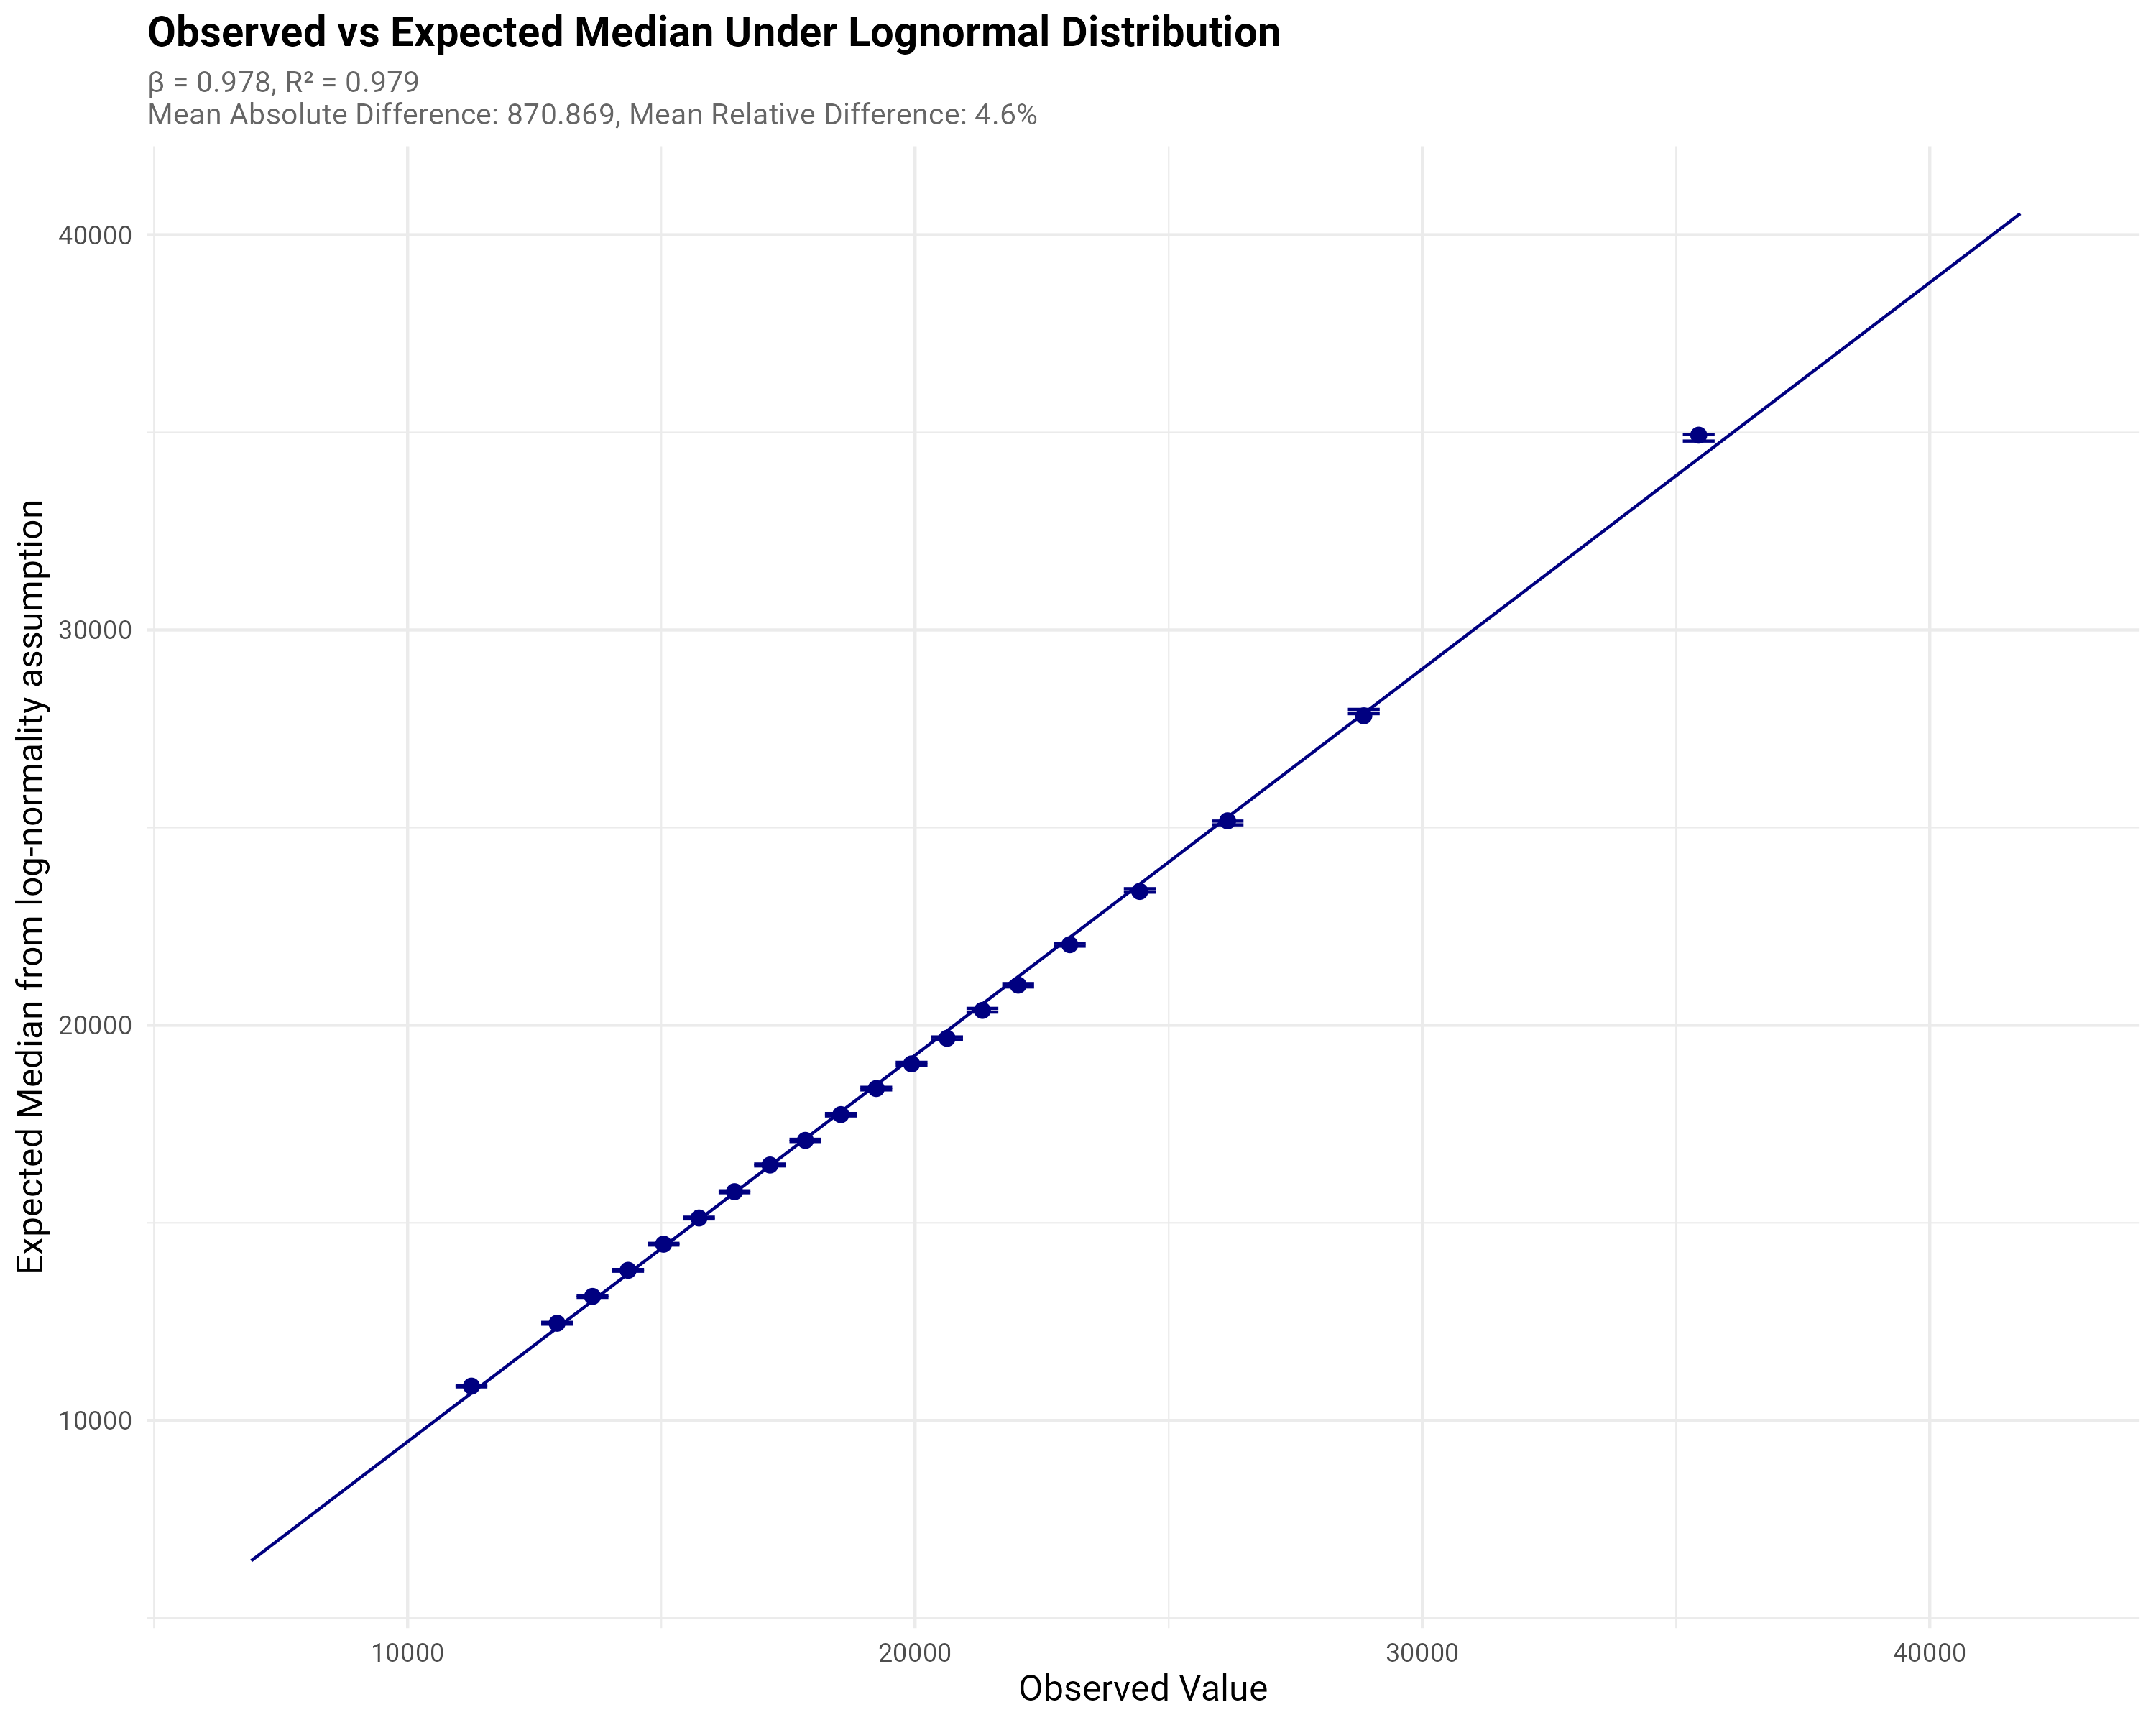
\includegraphics[width=0.9\textwidth]{output/binned_scatter_median.png}
\end{center}
\begin{fignotes}
\textbf{Notes:} This figure shows a binned scatter plot comparing observed median income with predicted values under the log-normal assumption for each census tract. 
\end{fignotes}
\end{figure}

Figure 2 shows the relationship for the P80/P20 ratio. The binned regression yields a slope coefficient of 1.09 ($R^2$ = 0.82), with predicted values deviating from observed ones by 5.0\% on average. The coefficient below unity suggests that the log-normal distribution slightly underestimates inequality in the tails, consistent with the fact that actual income distributions tend to have heavier tails.

\begin{figure}[H]
\begin{center}
\captionsetup{justification=centering}
\caption{Validation of log-normality: P80/P20 Ratio}
\label{fig:p80p20}
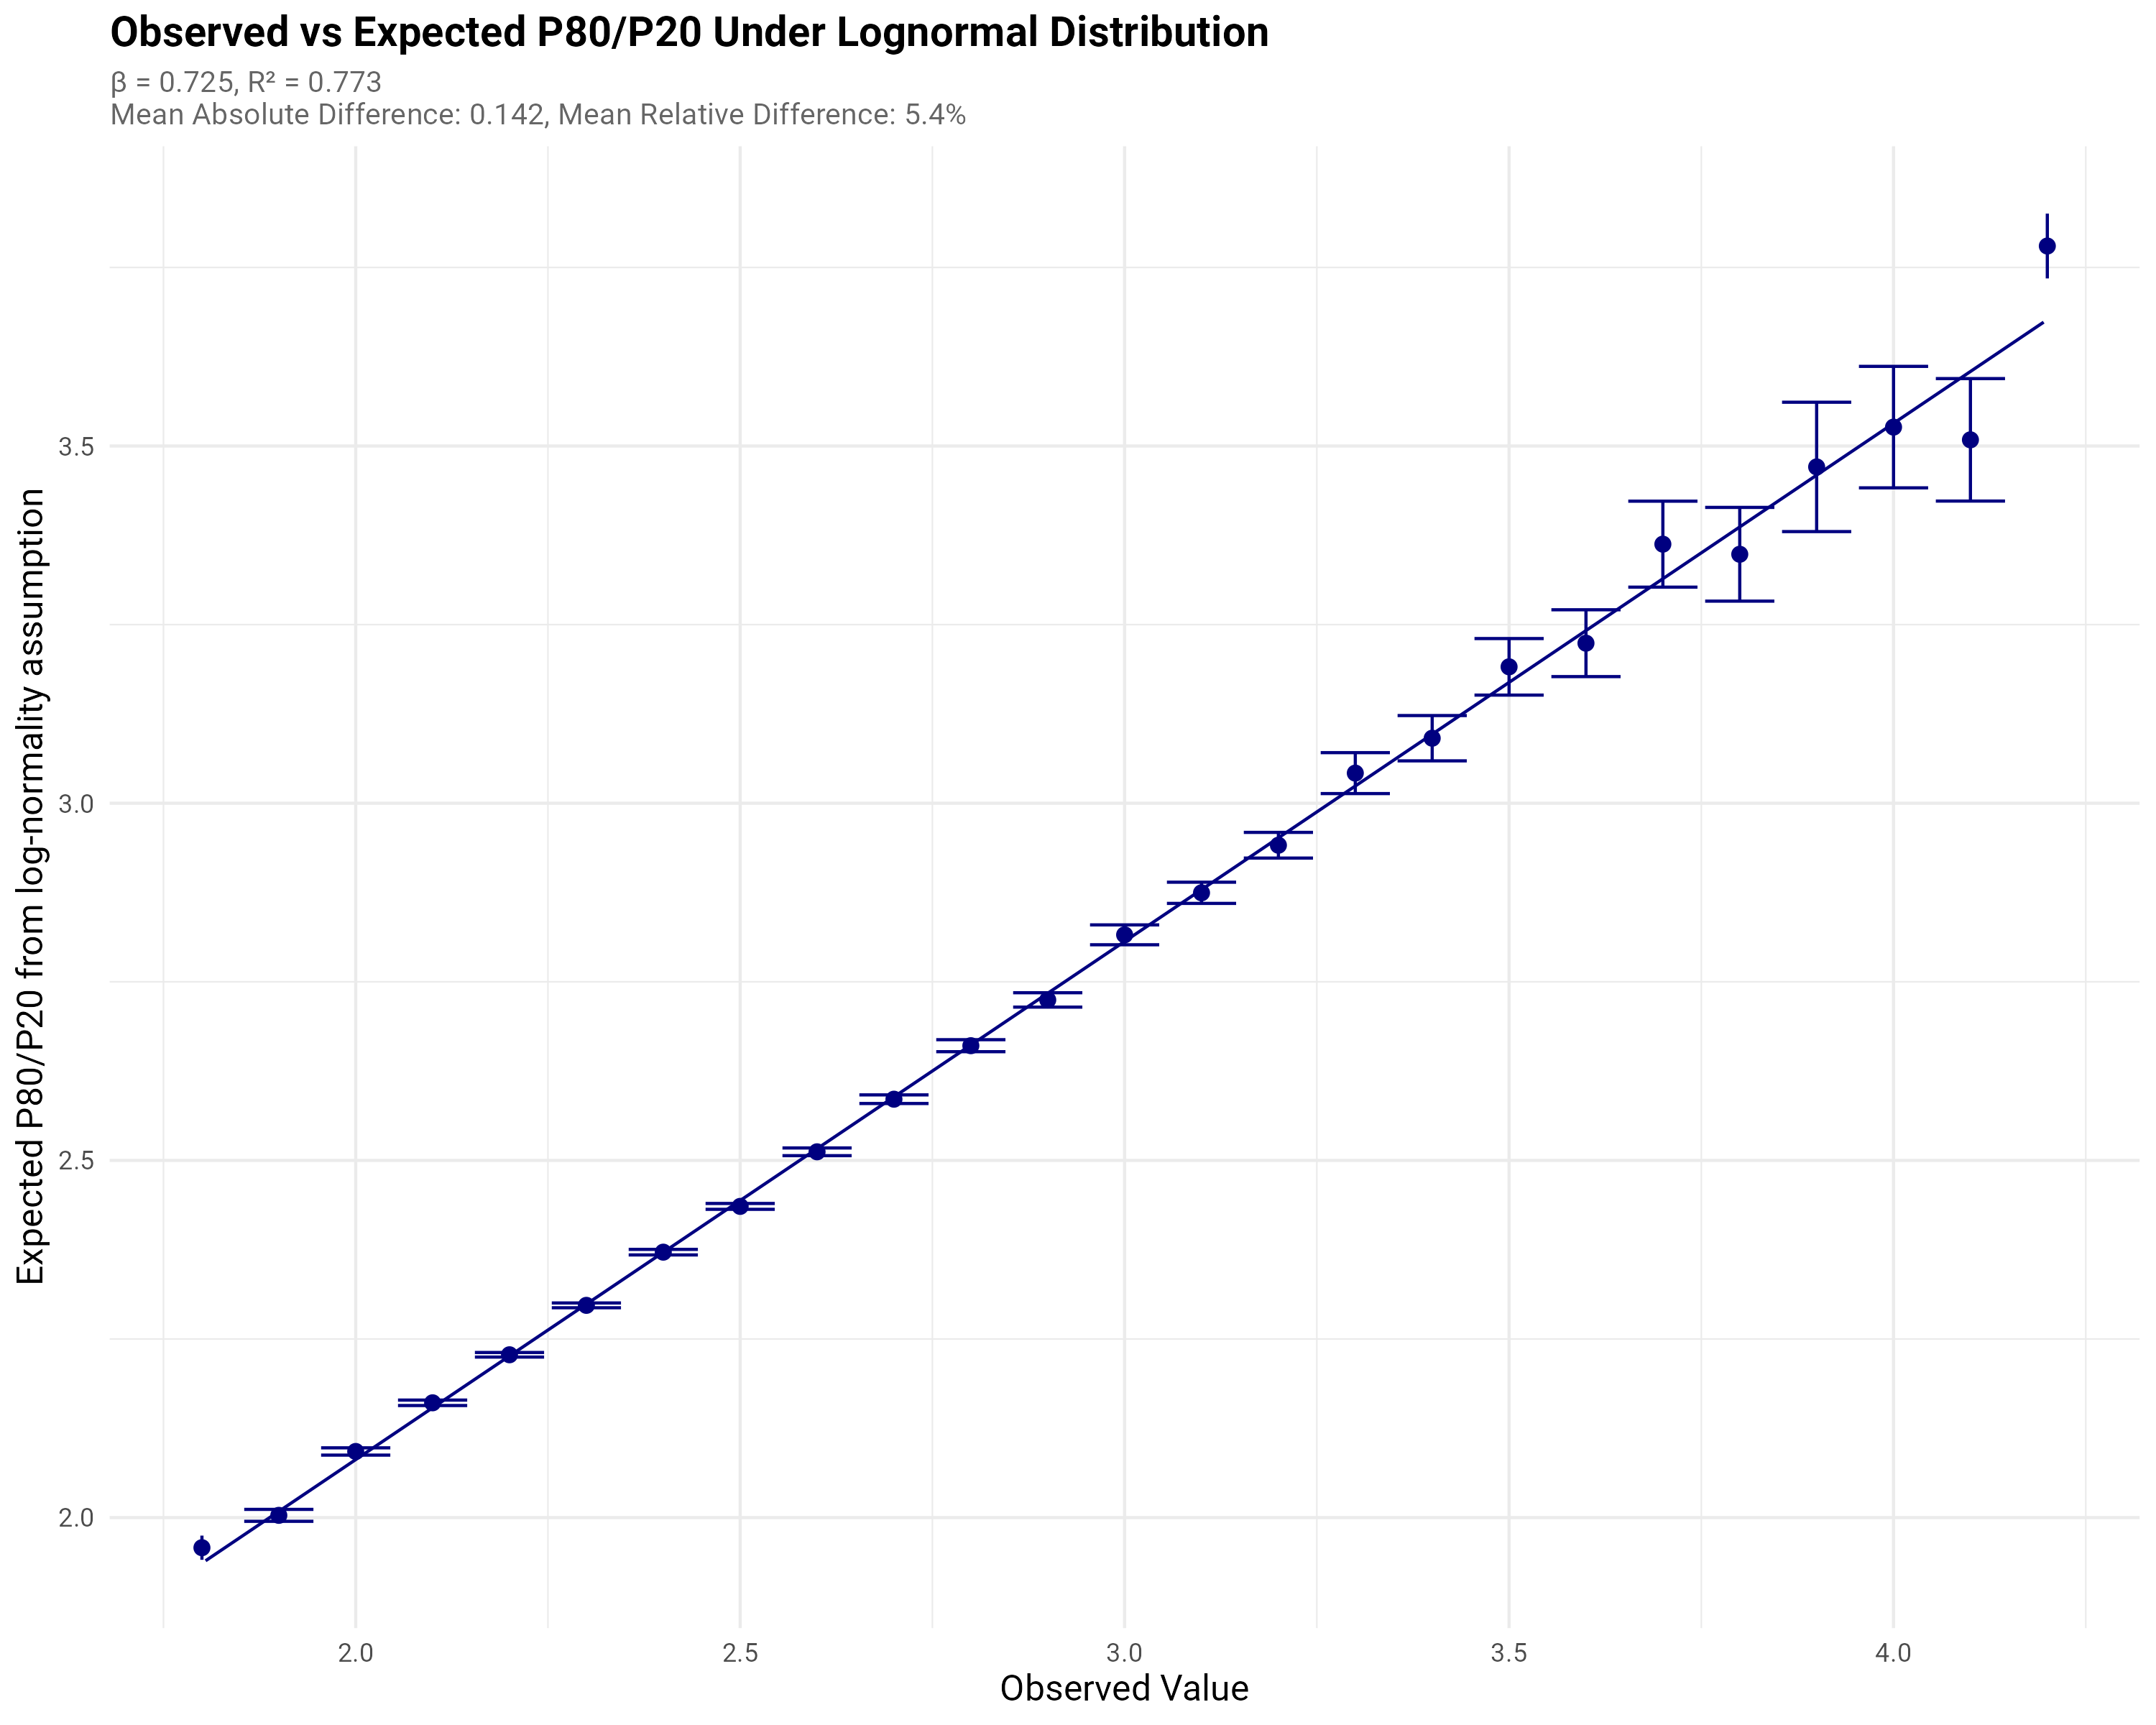
\includegraphics[width=0.9\textwidth]{output/binned_scatter_p80p20.png}
\end{center}
\begin{fignotes}
\textbf{Notes:} This figure shows a binned scatter plot comparing observed P80/P20 ratios with predicted values under the log-normal assumption for each census tract.
\end{fignotes}
\end{figure}